\section{Results: 500 MW, 100 km OWPP}

\begin{frame}{}
    \tableofcontents[currentsection]
\end{frame}

\begin{frame}{Random search vs NSGA-II}

\begin{figure}
    \centering
    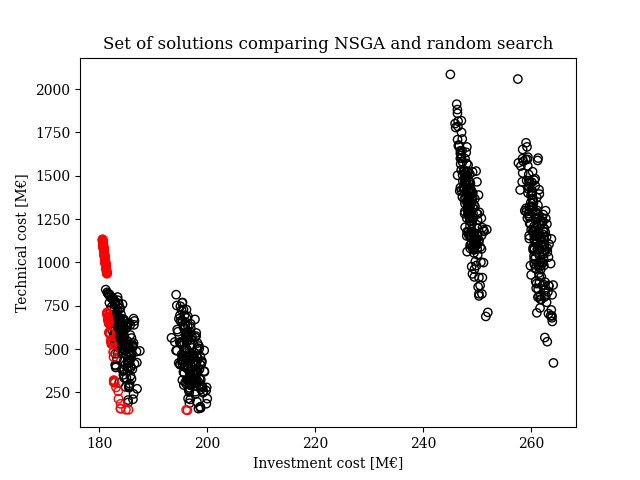
\includegraphics[width=0.65\textwidth]{imatges/random_vs_nsga_all.png}
    \caption{Random search (black) compared to NSGA-II (red).}
    \label{fig:random_search}
\end{figure}
    
\end{frame}

\begin{frame}{Zoom on Pareto Front}

    \begin{figure}
        \centering
        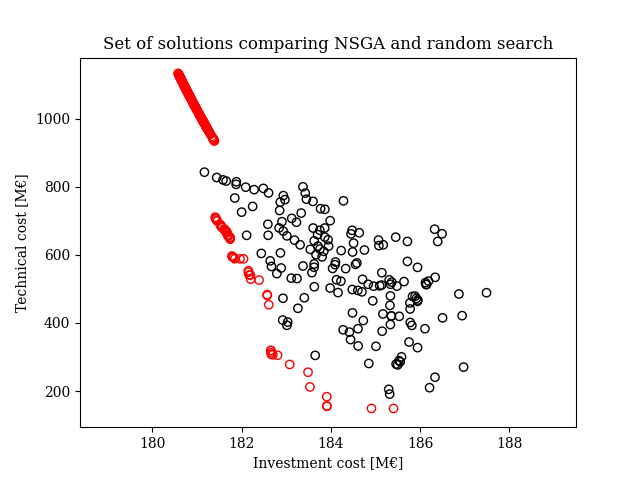
\includegraphics[width=0.65\textwidth]{imatges/random_vs_nsga_zoom.png}
        \caption{Zoom on Pareto Front, random search (black) compared to NSGA-II (red).}
        \label{fig:random_searchzoom}
    \end{figure}
        
    \end{frame}

\begin{frame}{OPF validation: Convergence}

It takes OPF about 1.5 s to converge, x25 slower than he traditional PF.
    \begin{figure}
        \centering
        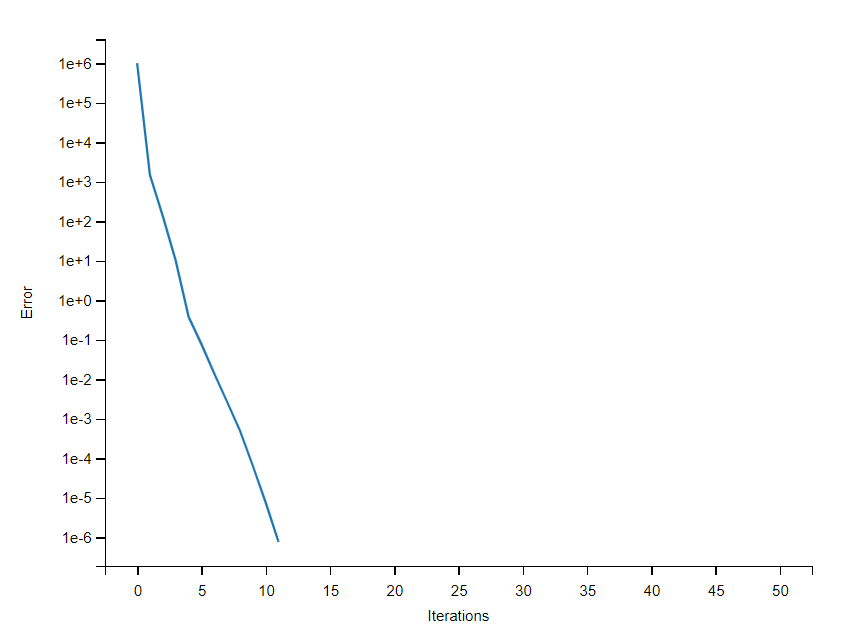
\includegraphics[width=0.65\textwidth]{imatges/opf_convergence.png}
        \caption{Convergence of the OPF algorithm.}
        \label{fig:convergence}
    \end{figure}
        
\end{frame}

\begin{frame}{OPF validation: Reactors sizing}

    \begin{figure}
        \centering
        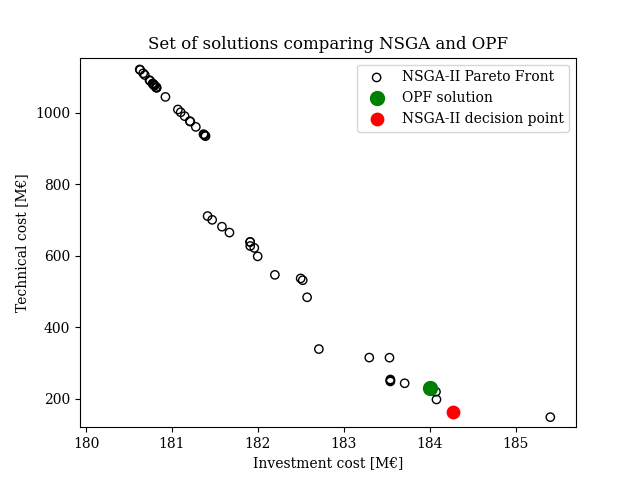
\includegraphics[width=0.65\textwidth]{imatges/opf_vs_nsga.png}
        \caption{NSGA-II vs OPF for reactors sizing}
        \label{fig:comparision}
    \end{figure}
        
\end{frame}

\begin{frame}{Costs comparision}
    \begin{figure}
        \centering
        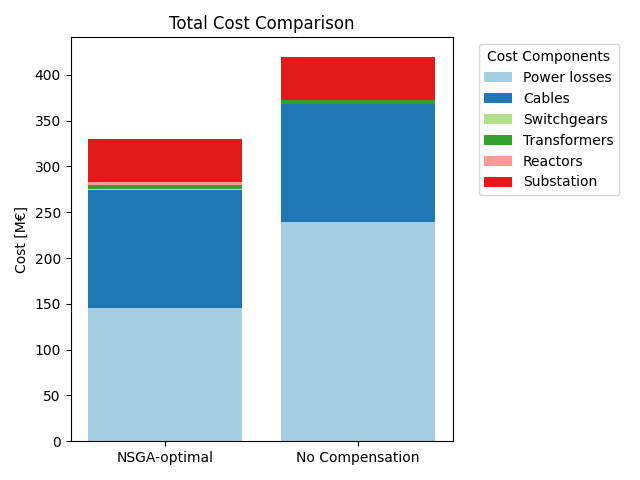
\includegraphics[width=0.65\textwidth]{imatges/cost_comparision.png}
        \caption{NSGA-II optimal solutions and no-compensation total cost comparision.}
    \end{figure}

\end{frame}

% \begin{frame}{Costs break Down}
% 
%     \begin{figure}[!htb]\centering
% 
%         \begin{subfigure}{0.55\textwidth}
%           \centering
%           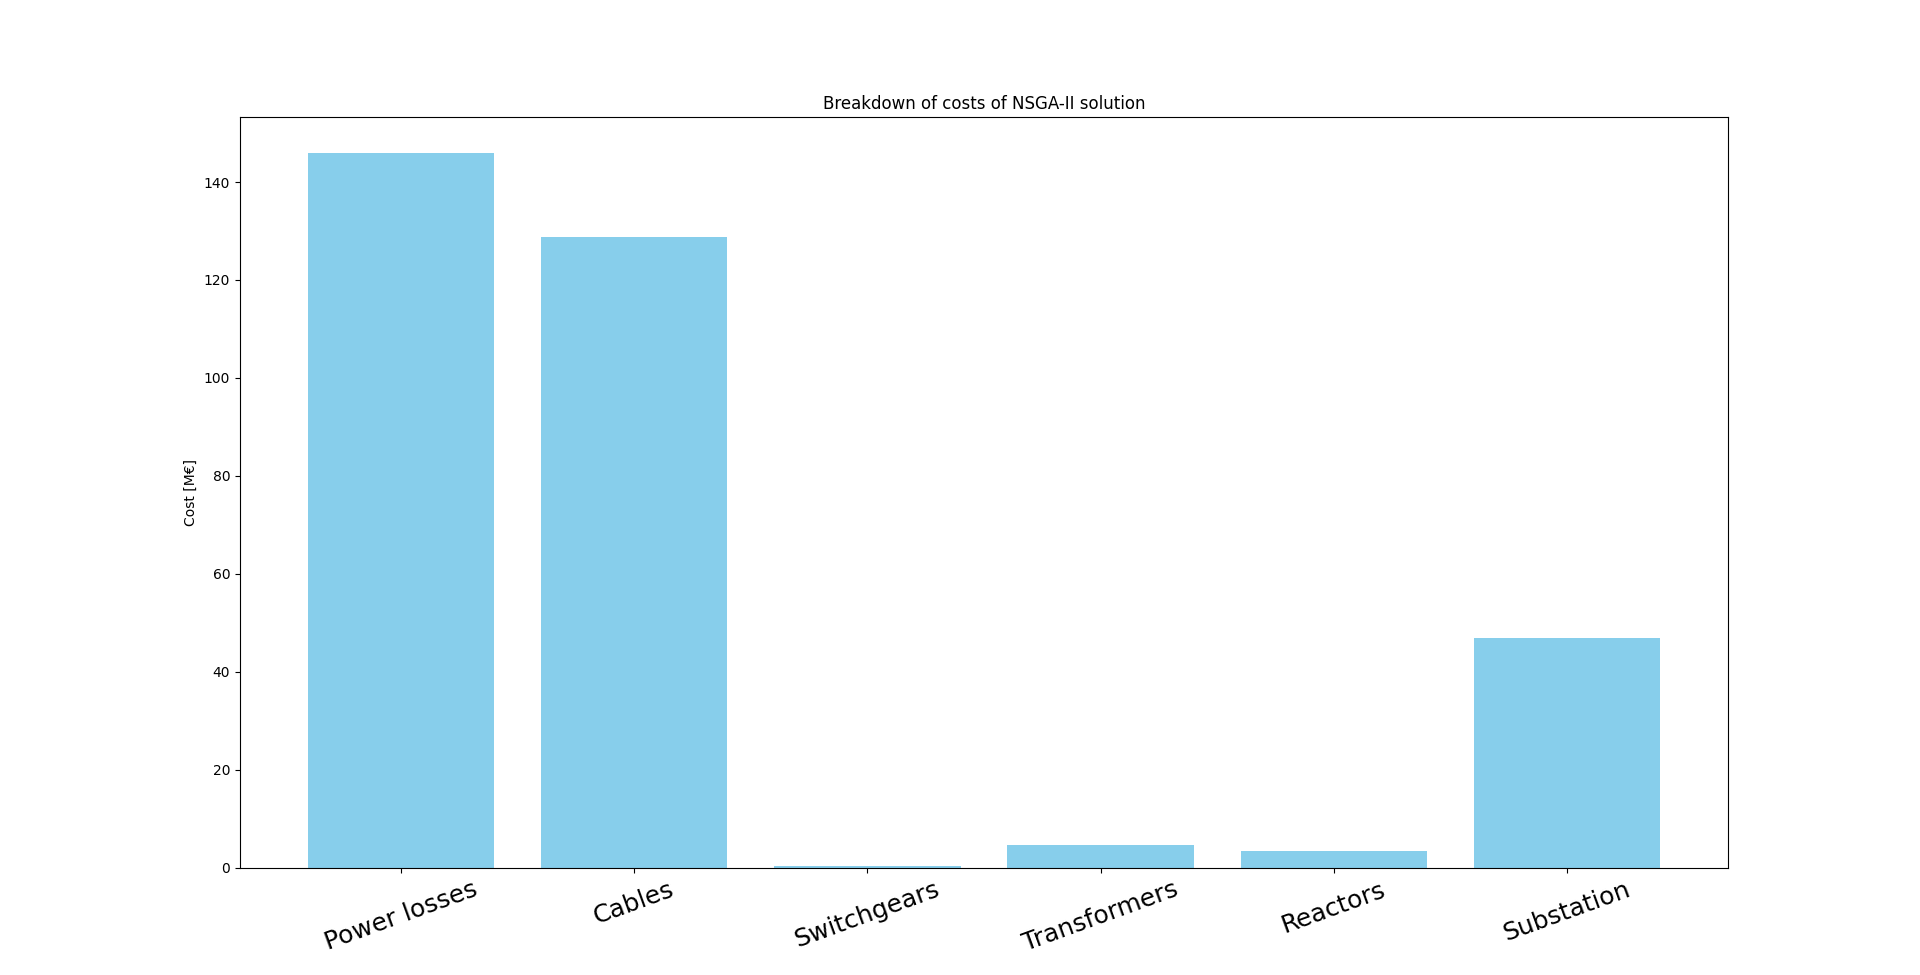
\includegraphics[width=6.0cm]{imatges/cost_nsga.png}
%           \caption{NSGA-II optimal solution costs.}
%         \end{subfigure}
% 
%     \vspace{5pt}
% 
%         \begin{subfigure}{0.55\textwidth}
%           \centering
%           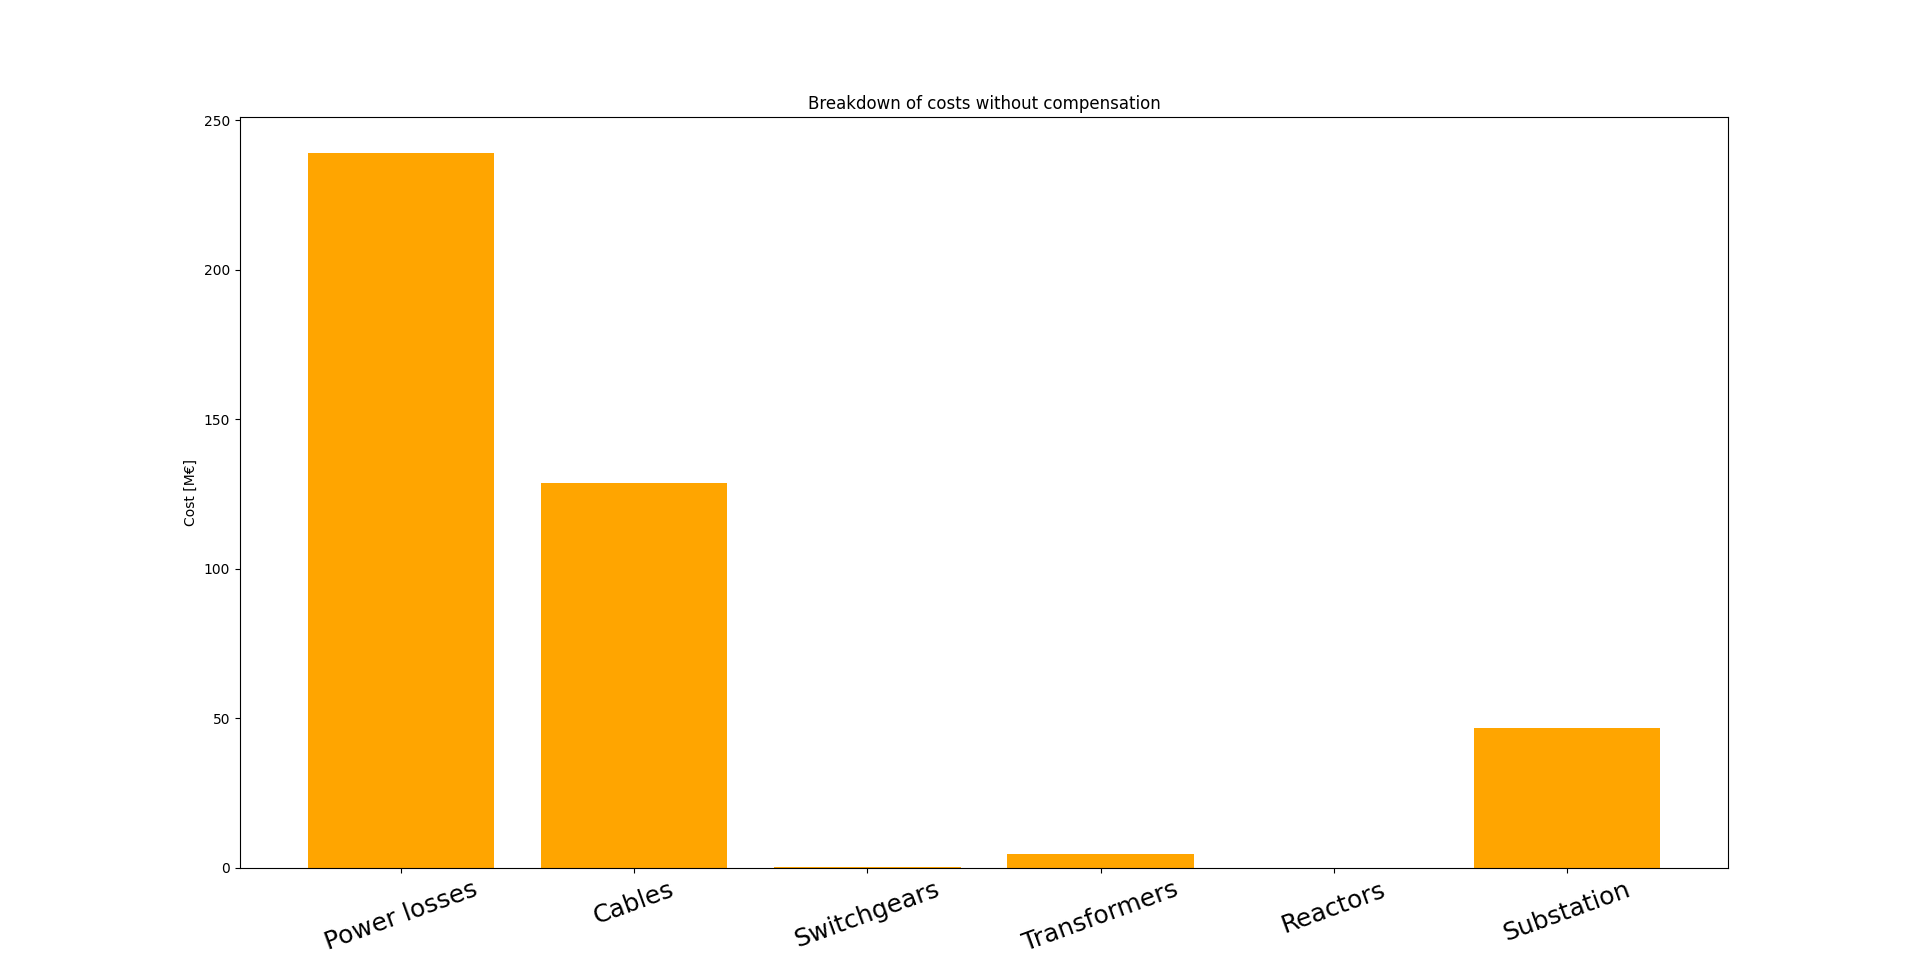
\includegraphics[width=6.0cm]{imatges/costs_nosh.png}
%           \caption{No compensation costs.}
%         \end{subfigure}
% 
% 
%       \end{figure}   
%         
% \end{frame}

\begin{frame}{Variable Power Injection: Power losses}
    \begin{figure}
        \centering
        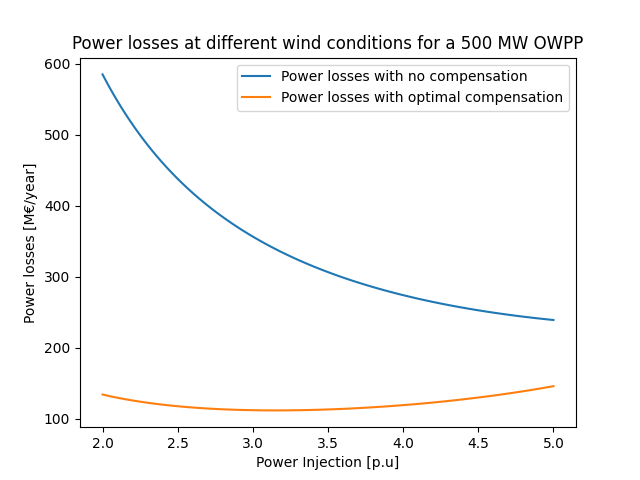
\includegraphics[width=0.65\textwidth]{imatges/losses evolution.png}
        \caption{Power losses evolution with variable $P_{owf}$.}
    \end{figure}

\end{frame}

\begin{frame}{Variable Power Injection: Overvoltages}
    \begin{figure}
        \centering
        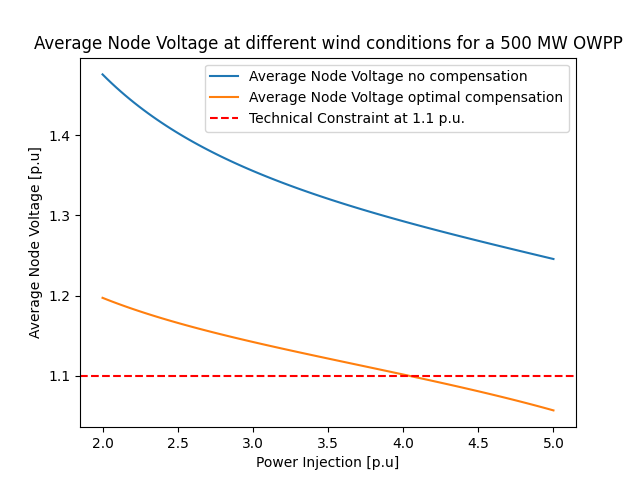
\includegraphics[width=0.65\textwidth]{imatges/overvoltageplot.png}
        \caption{Average Node voltage evolution with variable $P_{owf}$.}
    \end{figure}

\end{frame}


